\chapter{Конструкторская часть}

В данном разделе будут рассмотрены требования к программе и алгоритмы визуализации сцены и процесса водной эрозии.

\section{Требования к программному обеспечению}

Программа должна предоставлять следующие возможности:

\textbf{Динамическая визуализация процесса водной эрозии рельефа}:
\begin{itemize}
    \item исходная топография генерируется случайным образом;
    \item визуализация отображает изменения рельефа в реальном времени.
\end{itemize}

\textbf{Настройка физических параметров эрозии}:
\begin{itemize}
    \item возможность задания числа и шага итераций эрозии
    \item возможность изменения силы осаждения наносов и силы эрозии;
    \item возможность изменения числа капель.
\end{itemize}

\textbf{Реализация источника света}:
\begin{itemize}
    \item один источник света в сцене;
    \item возможность изменения интенсивности и цвета источника света.
\end{itemize}

\textbf{Графический интерфейс пользователя (GUI)}:
\begin{itemize}
    \item отображение результатов симуляции в реальном времени;
    \item инструменты для настройки параметров эрозии и освещения;
    \item возможность перезапуска визуализации.
\end{itemize}

\section{Описание структур данных}

Для формирования общего алгоритма синтеза изображения в данной
программе, необходимо ввести определения использующихся в ней структур
данных:

\textbf{Сцена:}
\begin{itemize}
    \item полигональная модель рельефа;
    \item модель эрозии;
    \item камера;
    \item источник освещения.
\end{itemize}

\textbf{Модель рельефа:}
\begin{itemize}
    \item массив вершин;
    \item массив полигонов;
    \item массив векторов нормалей.
\end{itemize}

\textbf{Камера:}
\begin{itemize}
    \item координаты положения в пространстве;
    \item координаты точки наблюдения;
    \item угол обзора
    \item ближняя и дальняя плоскости отображения;
    \item вектор ориентации.
\end{itemize}

\textbf{Источник освещения:}
\begin{itemize}
    \item координаты положения в пространстве;
    \item цвет;
    \item интенсивность.
\end{itemize}

\textbf{Модель эрозии:}
\begin{itemize}
    \item число итераций эрозии;
    \item шаг итераций;
    \item сила эрозии;
    \item сила отложения остатков;
    \item количество капель.
\end{itemize}

\section{Общий алгоритм синтеза изображения}

Визуализация сцены происходит поэтапно.
Описание алгоритма синтеза изображения представлено на рисунке~\ref{img:sint}.
На вход подаются параметры камеры и источника освещения.
На выходе -- синтезированное изображение.

\begin{figure}[H]
	\centering
	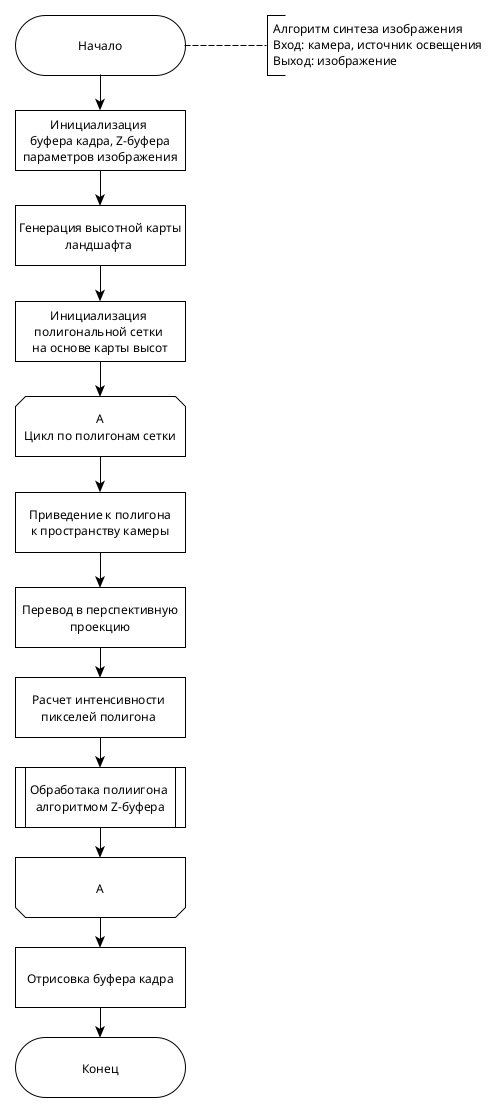
\includegraphics[scale=0.6]{images/sint}
	\caption{Описание алгоритма синтеза изображения}
	\label{img:sint}
\end{figure}

\section{Алгоритм Z-буфера}

Алгоритм Z-буфера используется для удаления невидимых поверхностей в процессе рендеринга сцены.
Он обеспечивает корректное отображение полигонов, скрывая те, которые находятся за другими объектами с точки зрения
наблюдателя. Описание алгоритма представлено на рисунке~\ref{img:zbuf_sch}.

\begin{figure}[H]
	\centering
	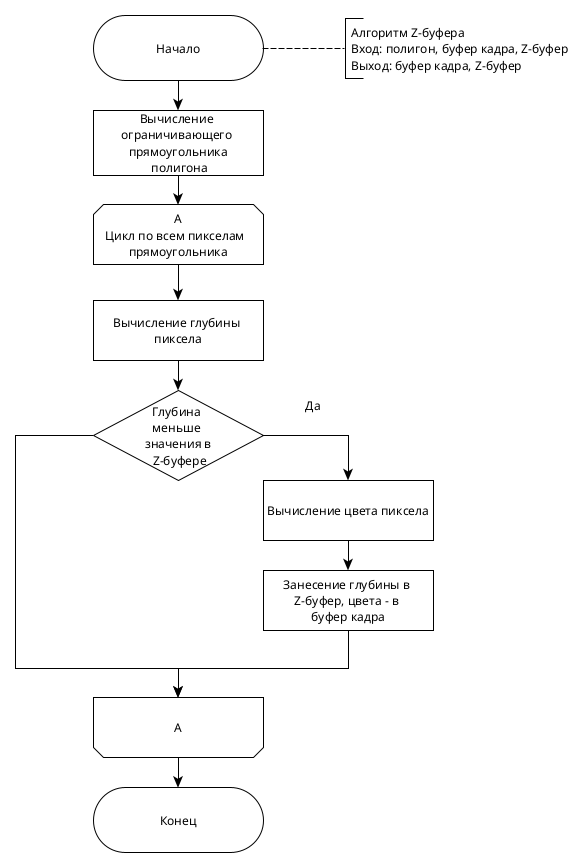
\includegraphics[scale=0.6]{images/zbuf_sch}
	\caption{Описание алгоритма Z-буфера}
	\label{img:zbuf_sch}
\end{figure}

\section{Алгоритм процесса эрозии на основе высотных карт}

Алгоритм гидравлической эрозии на основе высотных карт моделирует процесс размывания рельефа водой.
Он обновляет высотную карту рельефа в соответствии с физическими параметрами эрозии.
Описание алгоритма приведено на рисунках~\ref{img:erosion}~--~\ref{img:erosion2}.

\begin{figure}[H]
	\centering
	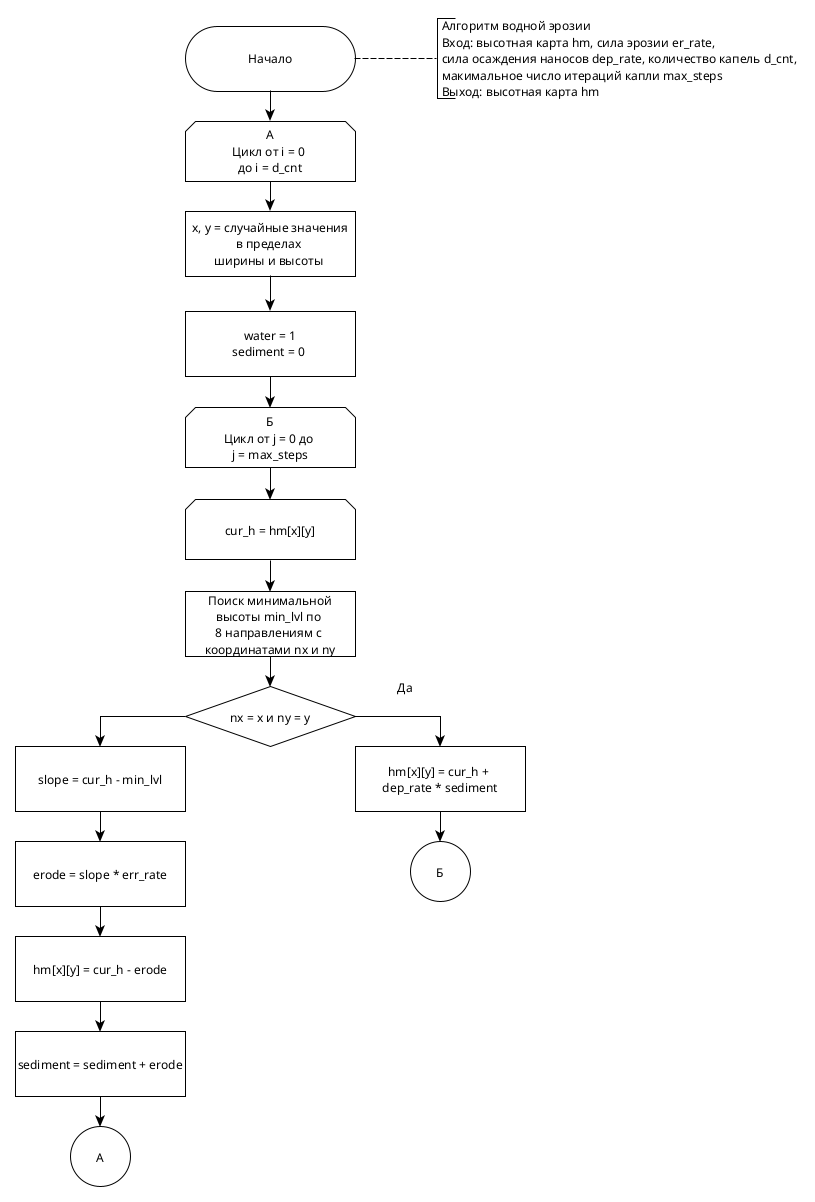
\includegraphics[scale=0.45]{images/erosion}
	\caption{Описание алгоритма водной эрозии}
	\label{img:erosion}
\end{figure}

\begin{figure}[H]
	\centering
	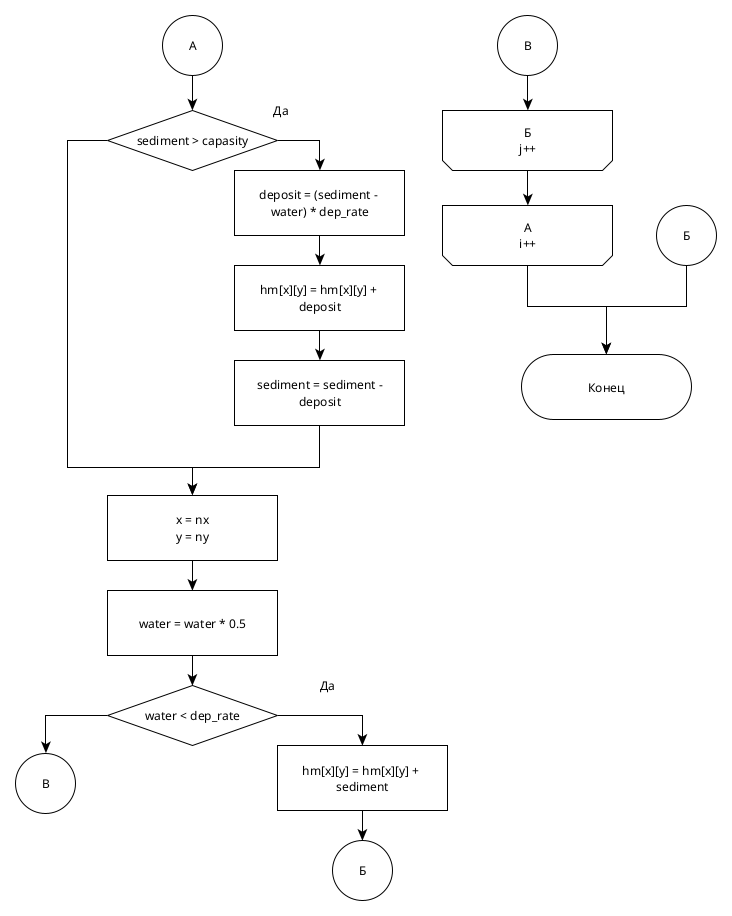
\includegraphics[scale=0.6]{images/erosion2}
	\caption{Описание алгоритма водной эрозии (продолжение)}
	\label{img:erosion2}
\end{figure}

Капля перемещается от высоких уровней к низким, забирая часть грунта.
Если у капли нет направлений для перемещения (впадина или плато)
или произошло ее испарение, часть переносимого грунта осаждается, размывая почву.

\section*{Вывод}

Были описаны требования к программному обеспечению, структуры данных и алгоритмы для построения сцены в
пространстве изображения.